%%
%% DOCUMENT TYPE
%%

% general options:
% - inputenc        file encoding (should be "utf8" in most cases)
% - de/en           language of your work (influence pre-defined tokens)
% - declaration     adds the mandatory statutory declaration for theses
% - abstract        adds the abstract (from file "prelude_abstract.tex")
% - acknowledgment  adds an acknowledgment (from file "prelude_acknowledgment.tex")
%                   it is a nice gesture to personally thank people who
%                   supported you during your work.
% - symbollist      adds a list of symbols (from file "prelude_symbols.tex")
% - figurelist      adds and automatically creates a list of figures 
% - tablelist       adds and automatically creates a list of tables
% - index           generates an index based on the package "makeidx", please
%                   refer to its documentation for usage on index markup
% - bibbacklinks    adds backlinks from bibliography to the pages, where the
%                   corresponding entry is used (cited)
% - gray            make a gray-style version of the thesis report
%
% PhD thesis specific options
% - cv              adds your cv
% - publishsize     changes the page size from A4 to A5 for print publishing
%                   (please change the font size to 9pt, if you use this option)
% - approved        use this option, after your thesis has been formally approved
%                   (this will change the front page to meet formal/legal requirements)
% - ownpub          adds a second bibliography (from file "ownpub.bib") for your own
%                   publications related to the PhD thesis. According to the latest
%                   examination regulations, own work should be part of the regular
%                   bibliography (this option is hence obsolete)

\documentclass[en,abstract,acknowledgment,symbollist,inputenc=utf8]{tuhhthesis}

\usepackage{tuhhlistings}


%%
%% SETUP BLOCK
%%

% thesis type, must be one of the following
% - projectwork
% - bachelorthesis
% - masterthesis
% - diplomathesis
% - phdthesis
\setthesistype{projectwork}

% your full name as printed on any official document (e.g., passport)
\author{Sergej Keller}

% the official title of your work (*must* match the filed title)
\title{Orthogonal Codes for Acoustic UnderwaterLocalization}

% the institution of the first examiner (refer to tuhhlangnames.def)
\institute{InstAutonomousCPS}

% date of submission as DD.MM.YYYY
\submitdate{01.04.2022}

% your matriculation number (for anything but PhD thesis)
\matrnumber{50484}

% PhD thesis only
%\setSexOfAuthor{male}
%\setBirthplace{Hamburg, Deutschland}
%\setPhDType{ing}

% your course of studies
\course{Informatik-Ingenieurwesen}

% full name and affiliation of first and second examiner
\examinerFirst{Prof. Dr.-Ing. Bernd-Christian Renner}{Institute of Autonomous Cyber-Physical Systems\newline Hamburg University of Technology}
\examinerSecond{Prof. Dr. Volker Turau}{Institute of Telematics\newline Hamburg University of Technology}

\supervisorFirst{Christoph Weyer}{Institute of Telematics, Hamburg University of Technology}
%\supervisorSecond{Volker Turau}{Institute of Telematics, Hamburg University of Technology}

% optional: print the TUB document number on title page
% this only applies, if the document is formally publish under
% a TUB document number
%\tubdoknumber{4711}


% Curriculum Vitae
% only needed for thesis type PhD
%\usepackage[]{currvita}
%\setlength{\cvlabelwidth}{50mm}
%\renewcommand*{\cvlistheadingfont}{\normalfont\sffamily\large\color{tuhh_blue}}
%\renewcommand*{\cvlabelfont}{\normalfont\rmfamily\normalsize\color{tuhh_darkgray}}



%%
%% CONTENT AREA
%%

% mathematical symbols
% absolute value, ceiling, floor
\newcommand{\abs}[1]{\left|{#1}\right|}
\newcommand{\floor}[1]{\left\lfloor{#1}\right\rfloor}
\newcommand{\ceil}[1]{\left\lceil{#1}\right\rceil}

% regular sets %
\newcommand{\setN}{{\mathbb N}}
\newcommand{\setZ}{{\mathbb Z}}
\newcommand{\setQ}{{\mathbb Q}}
\newcommand{\setR}{{\mathbb R}}
\newcommand{\setC}{{\mathbb C}}
\newcommand{\classNP}{{\cal {NP}}}
\newcommand{\classP}{{\cal {P}}}

% a node and a sink
\newcommand{\node}{v}
\newcommand{\sink}{\node_{0}}          % sink

% Node Related Sets
\newcommand{\Network}{G}
\newcommand{\setNodes}{{\mathcal V}}% set of nodes
\newcommand{\setLinks}{{\mathcal E}}% set of edges
\newcommand{\setNeighbors}[1]{{\mathcal N}_{#1}}% neighbors
\newcommand{\setTree}{{\mathcal T}}% tree
\newcommand{\setChildren}{{\mathcal C}}%
\newcommand{\setLeafs}{{\mathcal F}}%
\newcommand{\numNodes}{N}%
\newcommand{\numChildren}{C}%

% density
\newcommand{\nodeDensity}{\varrho}

%% EOF



\begin{document}


\chapter{PN and orthogonal sequences}

To attain a higher level of localization accuracy, there are two primary goals that must be pursued.\\
First, the code used for underwater localization should have an auto-correlation function that approaches a Dirac impulse. This is important because it allows for more efficient detection through the use of correlation techniques.\\
The second factor to consider is the cross-correlation properties of the code. It is essential that these attributes meet certain criteria in order to improve separation from other sequences. Mathematically speaking, this means that the codes should be orthogonal to each other, or at least approaching orthogonality. This will be particularly useful in real-world scenarios where noise, reflections, and other artifacts may be present.\\
In summary, by striving to achieve both of these objectives, it is possible to significantly improve the localization accuracy.

\section{Pseudo-random codes}

There are a couple of techniques to generate PN sequences. Most of these methods use linear feedback shift registers to generate the codes by an initial condition or seed value. In this project I will concertize my research on gold codes, kasami codes and the basic m-sequences which are used for generating gold codes. These types are all based on linear shift registers.\\
M-sequences are defined as binary PN codes, which are generated by linear shift registers with feedback. The sequences are periodic, and contain an equal number of zeros and ones \cite{proakis08}. 
Maximum length sequences need to fulfill certain criteria.  First its length is defined by $N=2^n - 1$ where $n$ is the maximum degree of the generator polynomial $f(X)$ \cite{sarwate80}.
 \begin{equation}
	 \lvert u\rvert=2^n-1=N,~~~\text{from polynomial}~~h(x) \text{of degree}~~n
\end{equation}
\begin{equation}
	\dfrac{N}{gcd(N,q)=N},~~~\text{from decimation polynomials}~~\widetilde{h(x)}
\end{equation}
Second the cross-correlation between m-sequences must take three values only, which are $-1$, $-t(n)$, $t(n) - 2$. With it $t(n)$ is defined by $1+2^{\lfloor0.5(n+2)\rfloor}$ \cite{sarwate80}.
If every pair of m-sequences is a preferred pair, they form a maximal connected set and these sets have a limited carnality. Experiments from Gold and Koptizke showed that the number of such connected pairs is limited. Between degrees $$$$ \cite{gold65}. To get an m-sequence we need a primitive polynomial. 

%\fignoframe{images/lfsr}{Basic structure of an LFSR (Linear Feedback Register). \cite{proakis08}}{fig:framelessFigures}

\subsection{Gold Codes}

Because of not optimal cross-correlation properties m-sequences alone are not applicable for the project. But if these type of codes are combined their correlation qualities can change. Gold Codes are m-sequences where two of them with same length are modulo-2 summed. \cite{proakis08} \\
Recent research shows that some gold codes have high similarity to a Gaussian random variable \cite{merrifield}. 

\begin{equation}
Gold(u,v)=\{u,v,u\oplus v,u\oplus(v \ll1),\dots,u\oplus(v\ll N-1)\}
\end{equation}

%\fignoframe{images/gold}{LFSR structure of preferred generator polynomial of degree 13. \cite{merrifield}}{fig:framelessFigures}

\subsection{Kasami Codes}

Kasami sequences are constructed in the similar fashion by using m-sequences with the exception that a second sequence, which is used in the modulo sum, is formed by decimating the default m-sequence by  $2^{m/2}$ \cite{proakis08} \cite{sarwate80} \cite{peterson72}. Thus, only one generator polynomial is required.

\begin{equation}
w=u[2^{N/2}+1]=\{u_1,\dots, u_i, \dots,u_{N}|\text{take every }i\text{-th bit of u}\} 
\end{equation}
\begin{equation}
Kasami(u)=\{u,u\oplus w,u\oplus(w \ll1),\dots,u\oplus(w\ll2^{N/2}-2)\}
\end{equation}


\section{Comparison}


For the localization process by orthogonal codes certain criteria needs to be met, which were named in the first chapter. To compare the before explained code types three measures are introduced. \\ 
The first one is the peak to side-lobe ratio (PSR) \ref{eq:psr}. This measure is defined by subtracting the mean from the peak of the auto-correlation. Then this value get divided by the standard deviation of the same auto-correlation. A higher PSR value signifies a lower error between the auto correlation and the perfect Dirac resulting in better detection capability. The second one is the ratio between the auto-correlation peak and the maximum of the cross-correlation (ACR) \ref{eq:acr}. There a higher value indicates good code separation qualities.\\
The comparison is done by sampling pairs at degrees six to ten $N$ times from the set of random sequences. These pairs are then used for generating the wanted pseudo-random codes like gold or kasami. Afterwards for all three code types the shown measures are applied.  

%The last one is the correlation coefficient showing if there are similar anchros \ref{eq:coeff}, which would be a bad indicator.

\begin{equation}
PSR=\dfrac{max\{x_{ac}\}-\overline{x_{ac}}}{\sigma_{ac}}
\label{eq:psr}
\end{equation}

\begin{equation}
ACR=\dfrac{max\{x_{ac}\}}{max\{{x_{cc}\}}}
\label{eq:acr}
\end{equation}

%\begin{equation}
%\rho(a1,a2)=\dfrac{cov\{a1,a2\}}{\sigma_{a1}\cdot\sigma_{a2}}
%\label{eq:coeff}
%\end{equation}
%\begin{figure}[h]
%	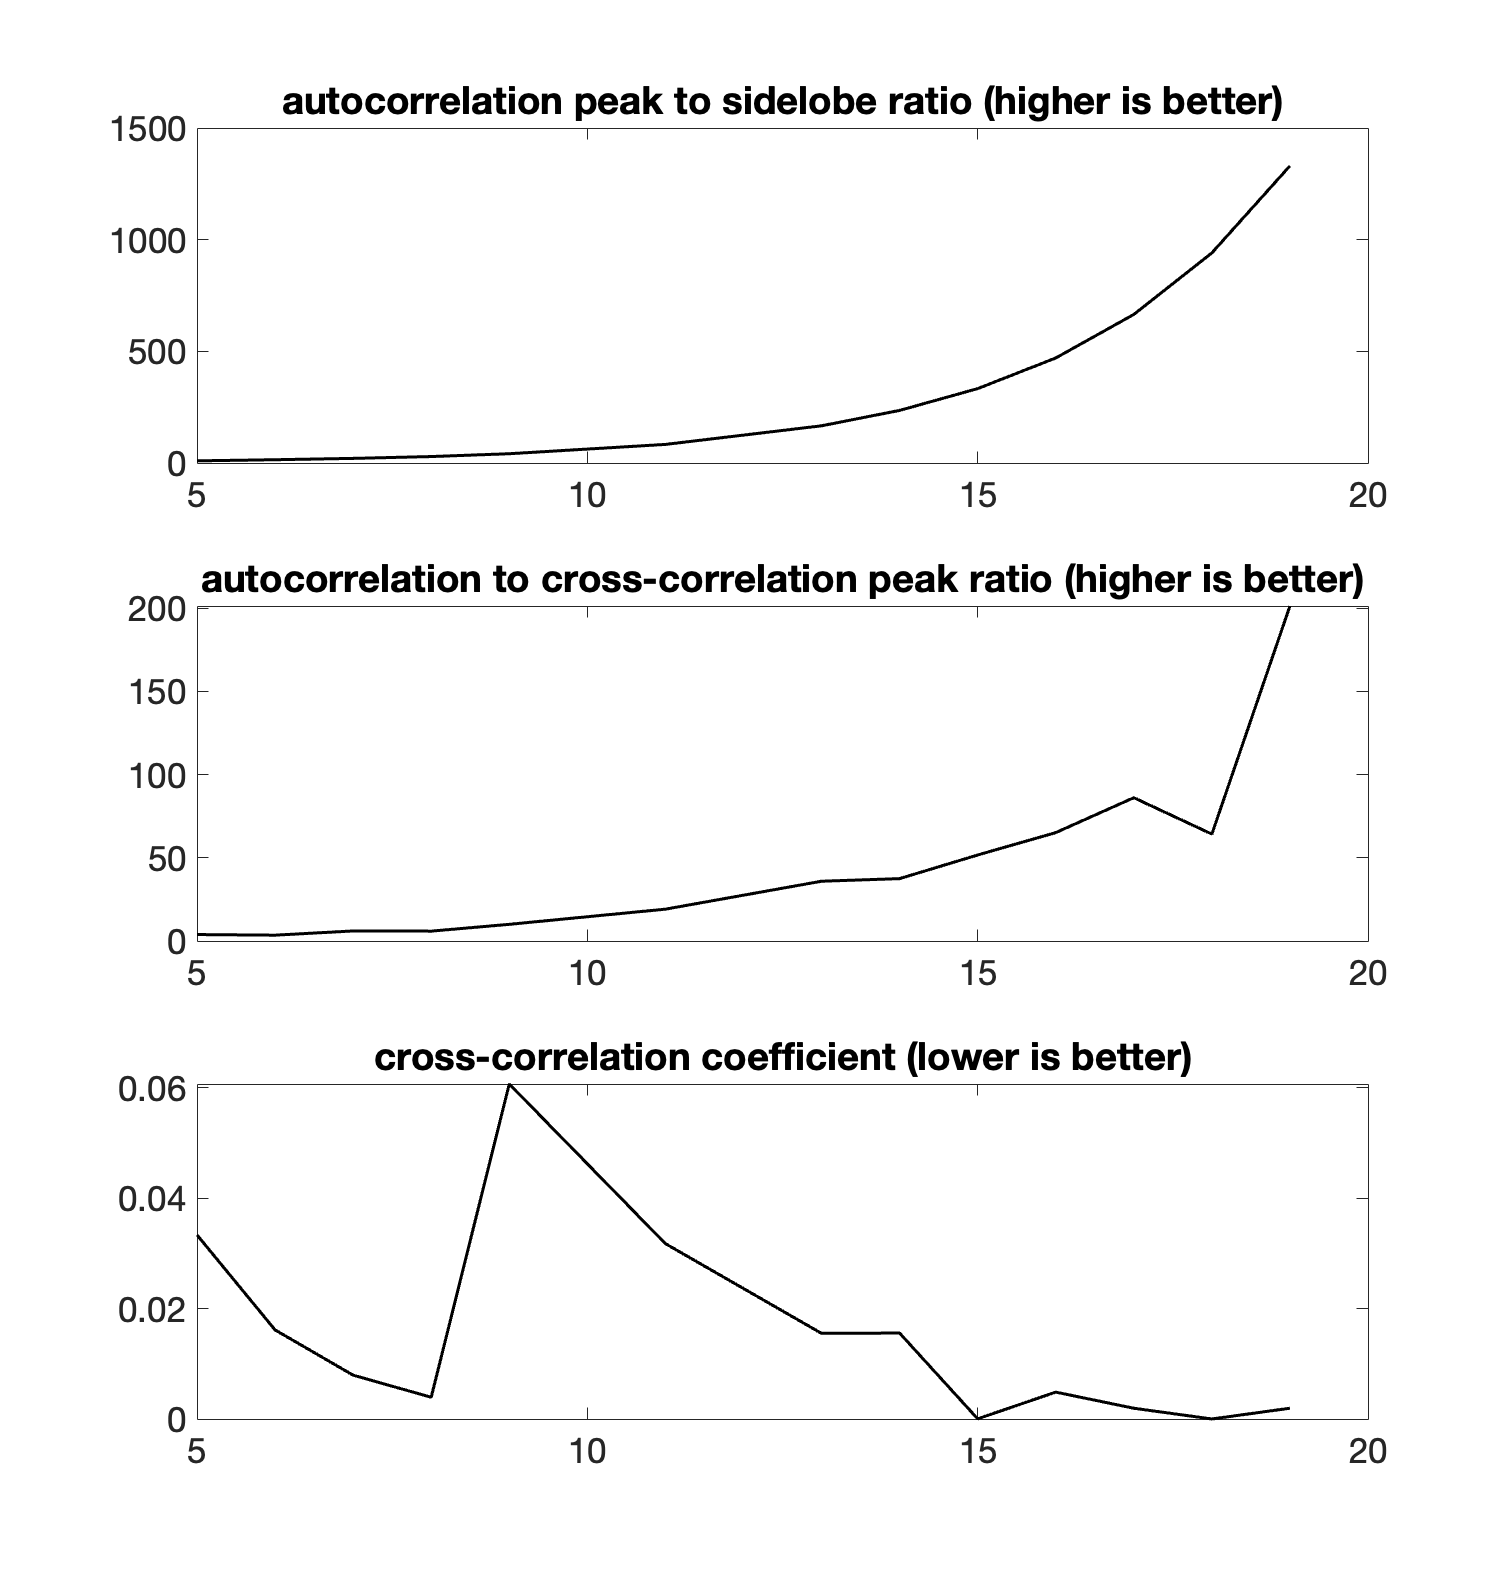
\includegraphics[width=8cm]{images/matlabplots/mseq}
%
%	\caption{Maximum Length Sequence evaluation}
%\end{figure}
%
%\begin{figure}[h]
%	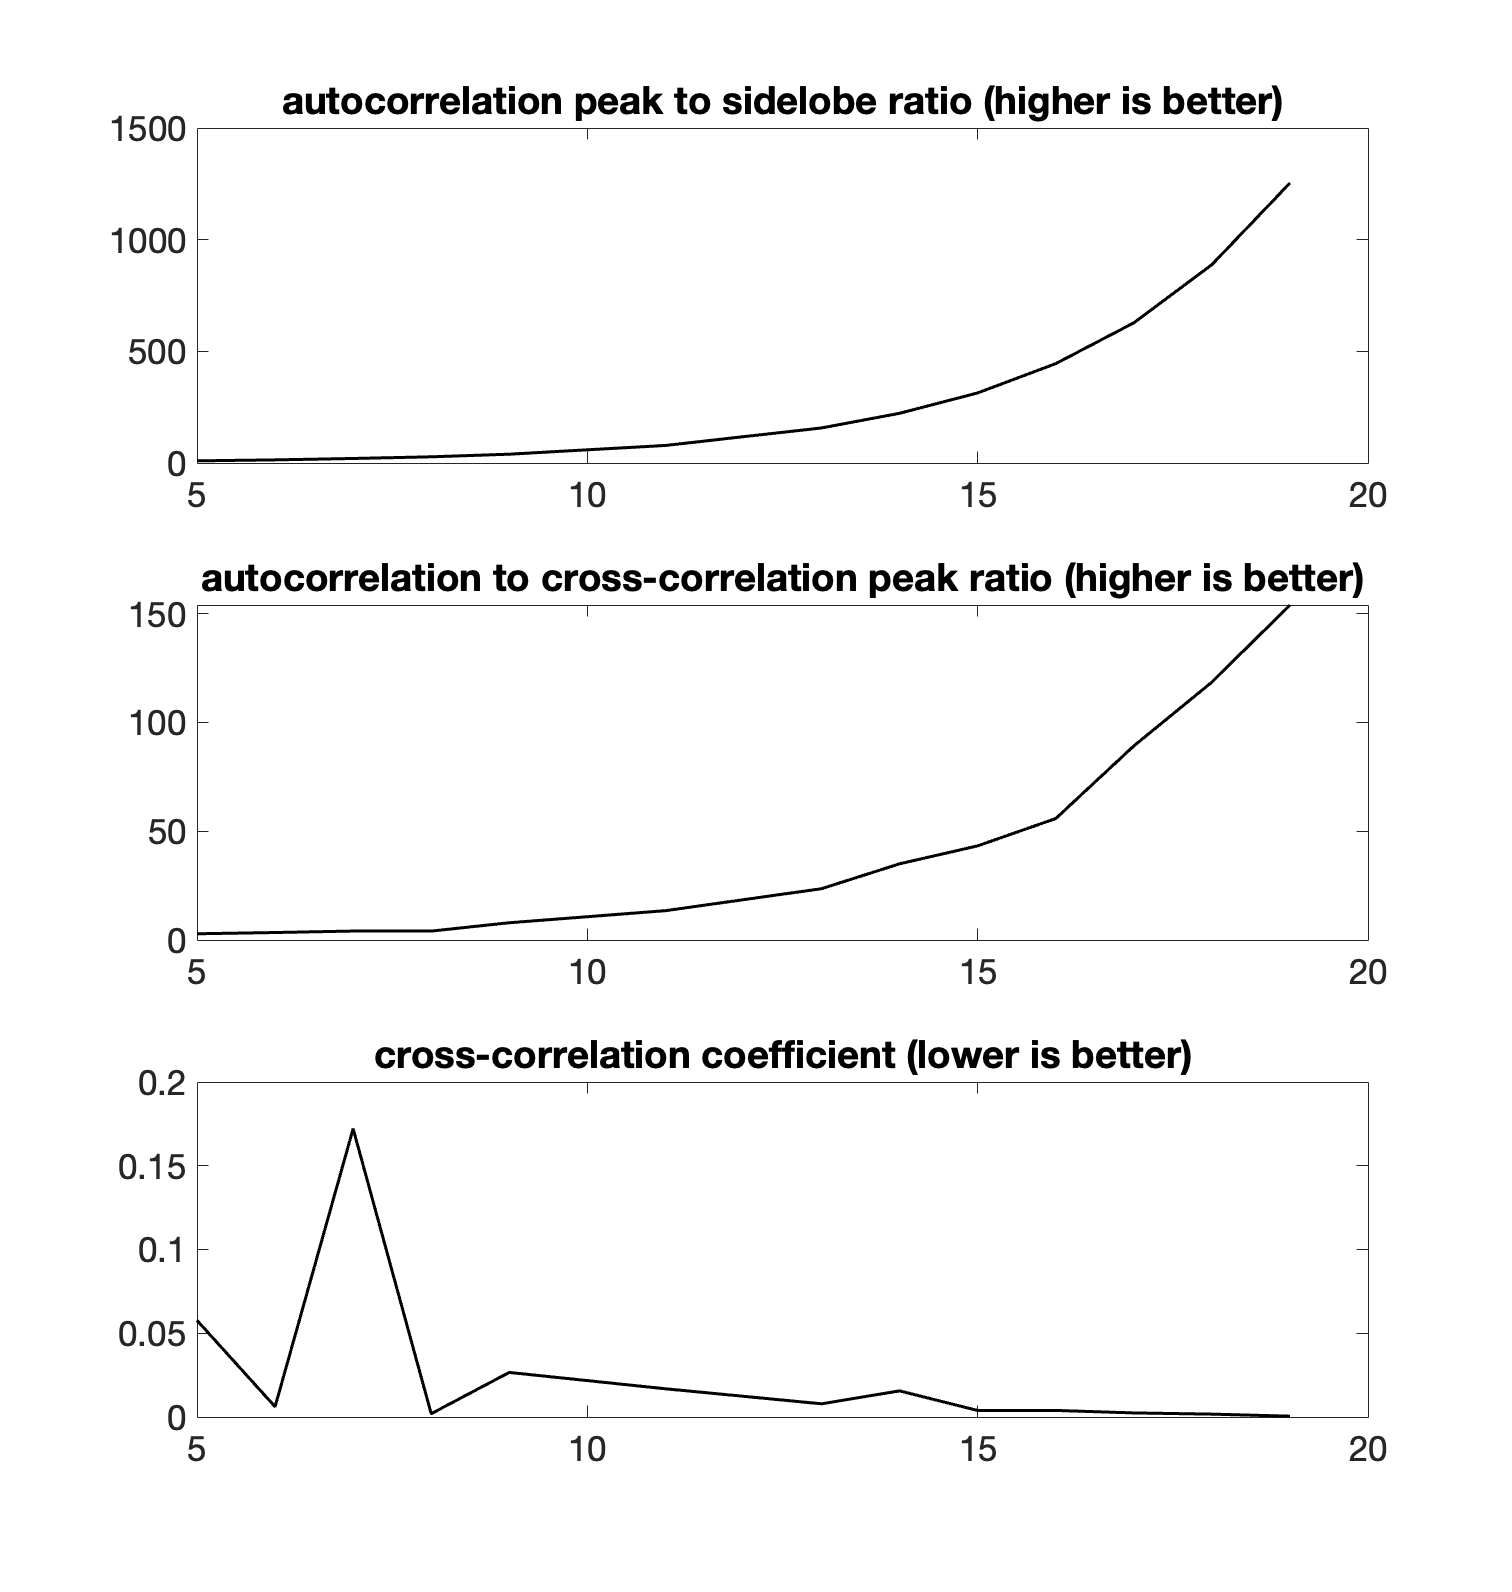
\includegraphics[width=8cm]{images/matlabplots/gold}
%
%	\caption{Gold sequence evaluation}
%\end{figure}
%
%\begin{figure}[h]
%	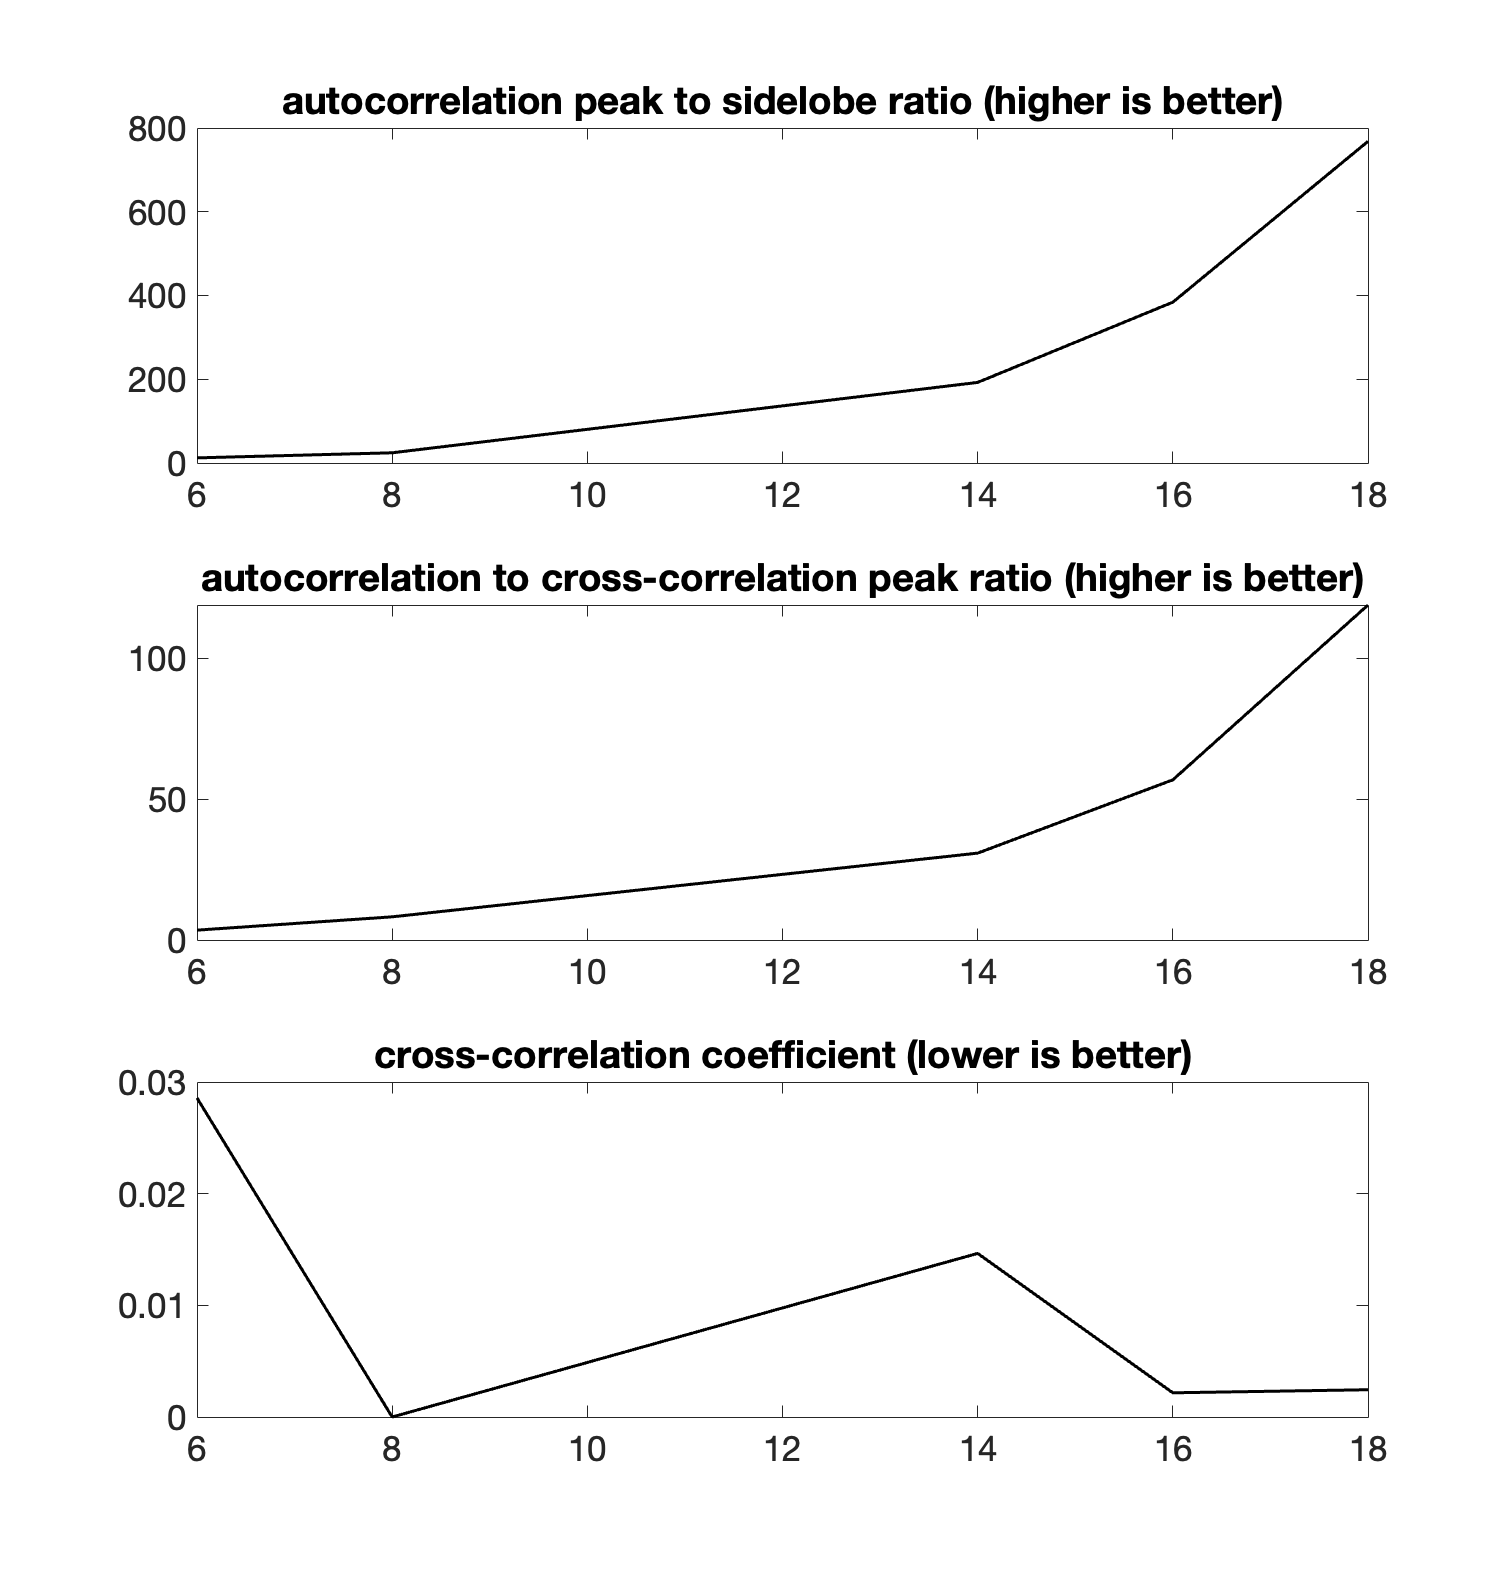
\includegraphics[width=8cm]{images/matlabplots/kasami}
%
%	\caption{Kasami sequence evaluation}
%\end{figure}
%%\fignoframe{images/matlabplots/mseq}{Basic structure of an LFSR (Linear Feedback Register). \cite{proakis08}}{fig:framelessFigures}
%%\fignoframe{images/matlabplots/gold\_10ms}{Basic structure of an LFSR (Linear Feedback Register). \cite{proakis08}}{fig:framelessFigures}
%%\fignoframe{images/matlabplots/kasami\_10ms}{Basic structure of an LFSR (Linear Feedback Register). \cite{proakis08}}{fig:framelessFigures}
%\section{Results}
In this evaluation of data, three types of codes were compared. Maximum length sequences, Gold Codes, and Kasami Codes. The performance of each code was assessed using two ratios, the ACR and the PSR.\\
From preferred polynomial all possible maximum length sequences, gold sequences and kasami sequences are generated. Then both measures are applied on the cross-correlation and auto-correlation functions of the random codes. The PSR and ACR measures are plotted against the used polynomials. Also the best case of PSR and ACR are plotted by their given correlation function.\\
Maximum length sequences hold the best auto-correlation properties in comparison to its competitors. But it shows peaks in its cross-correlation, making it a rather bad option for orthogonal separation. The kasami sequence has a way better cross-correlation but still a small peak. The clear winner are gold codes because of the good auto-correlation and very good cross-correlation properties \ref{fig:eva}. Its auto-correlations lags a bit behind its competitors but orthogonality is as much as important. 
%
%\begin{figure}[h]
%	\centering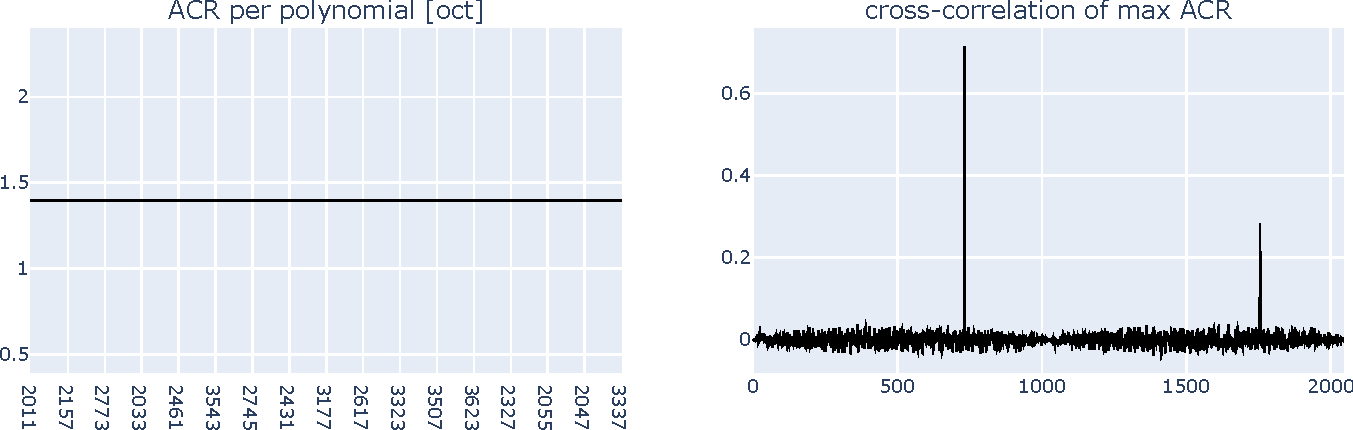
\includegraphics[width=13cm]{images/mseqevaacr}
%	
%	\caption{Evaluation of m-sequences by AC ratio}
%	\label{fig:eva}
%\end{figure}
%
%\begin{figure}[h]
%	\centering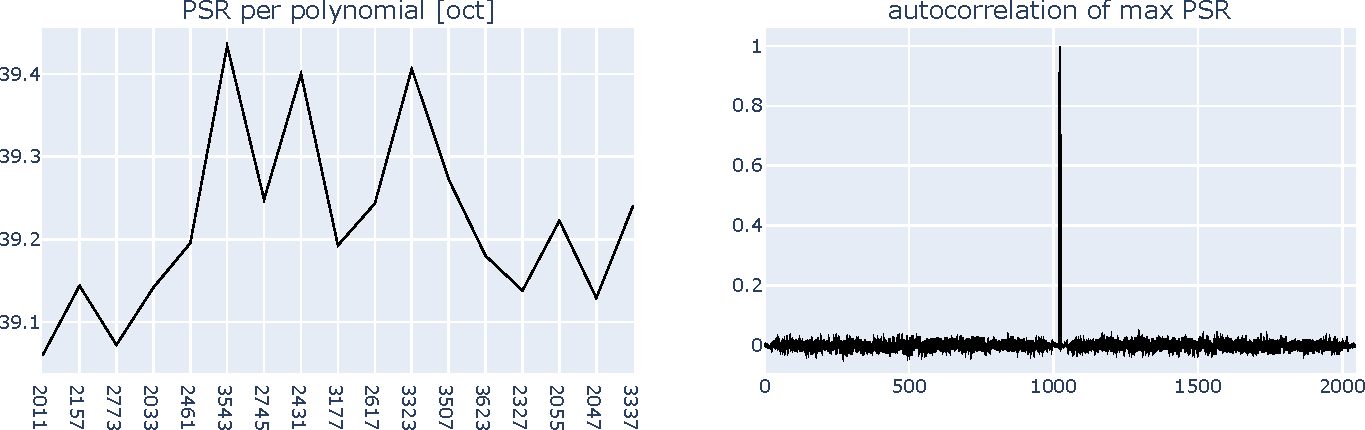
\includegraphics[width=13cm]{images/mseqevapsr}
%	
%	\caption{Evaluation of m-sequences by PS ratio}
%	\label{fig:eva}
%\end{figure}

\begin{figure}[h]
	\centering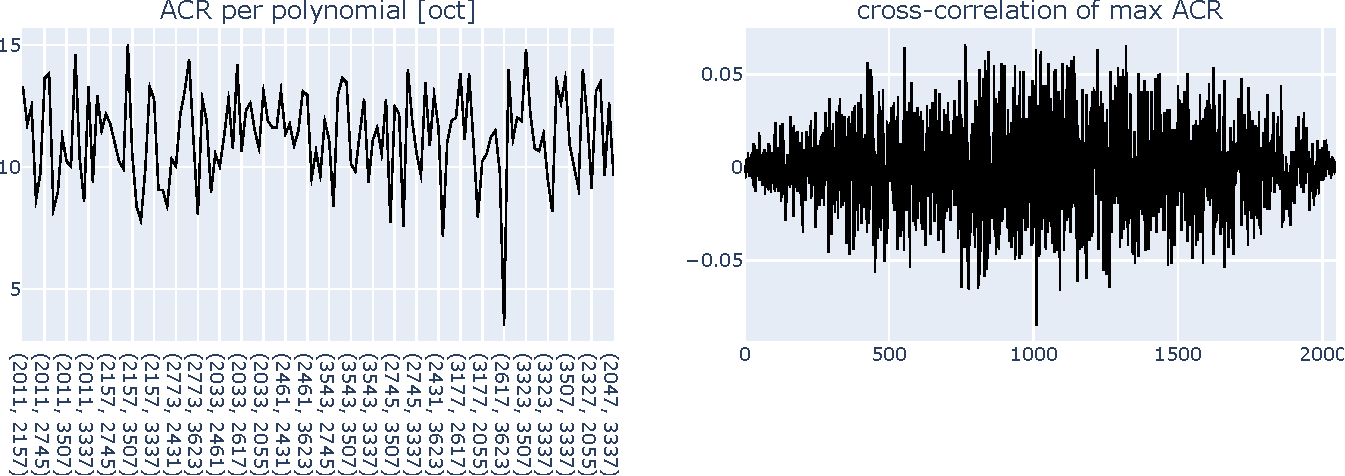
\includegraphics[width=14cm]{images/goldevaacr}
	
	\caption{Evaluation of gold sequences by AC ratio}
	\label{fig:eva}
\end{figure}

\begin{figure}[h]
	\centering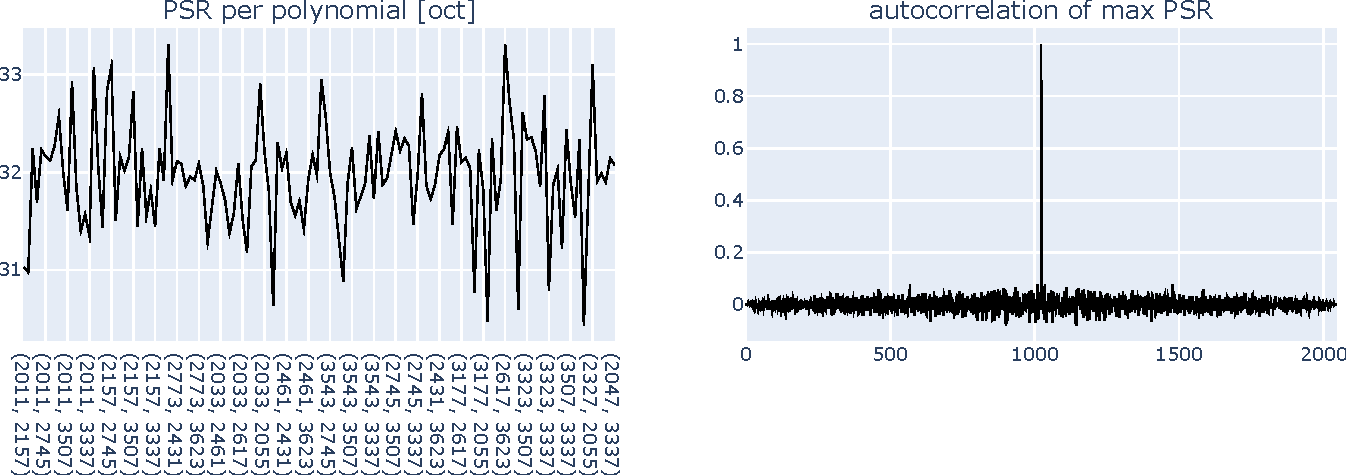
\includegraphics[width=14cm]{images/goldevapsr}
	\caption{Evaluation of gold sequences by PS ratio}
	\label{fig:eva}
\end{figure}
To get more valuable data, elements from each set of codes are sampled uniformly ($N=1000$) and afterwards the evaluation parameters are applied.
The results yields that Gold Codes had the least increase in PSR, but were the second best at ACR. Kasami Codes were only slightly better in both PSR and ACR than Gold Codes, but had a smaller set of codes available. Maximum length sequences had the highest PSR, but the worst ACR.\\
Based on these findings, it can be concluded that Gold Codes are the best choice for this application. While maximum length sequences had the highest PSR, they performed poorly in terms of ACR. Gold Codes, on the other hand, had a good balance of performance in both ratios, and also had a large set of codes available. In addition, Gold Codes demonstrated better cross-correlated detection compared to maximum length sequences.
\begin{figure}[h]
	\centering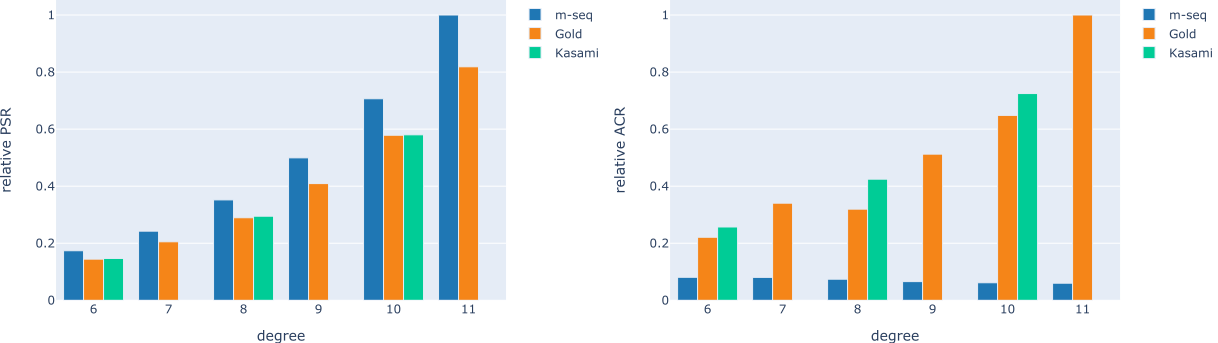
\includegraphics[width=14cm]{images/degCompEva}
	
	\caption{Evaluation by relative PSR for degrees 6 to 11}
	\label{fig:eva}
\end{figure}

%\begin{figure}[h]
%	\centering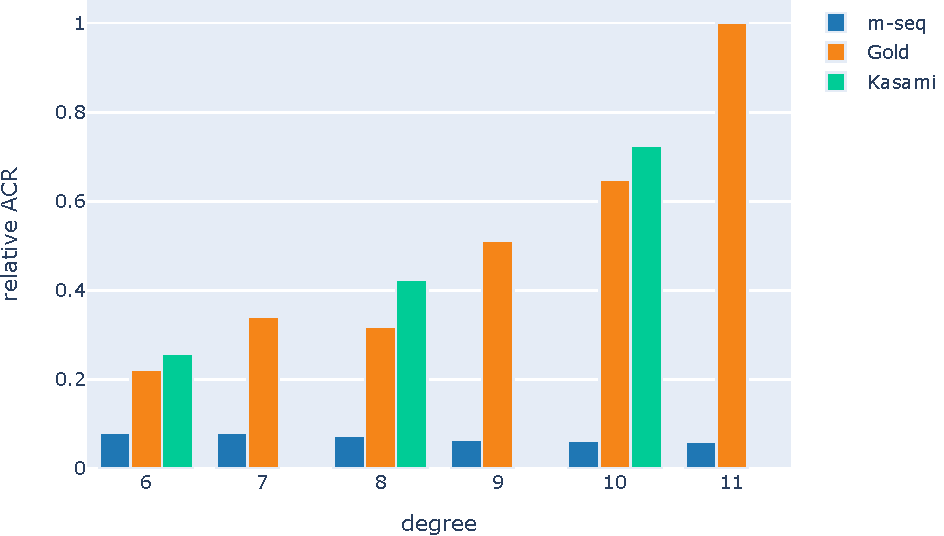
\includegraphics[width=13cm]{images/degAcrEva}
%	
%	\caption{Evaluation by relative ACR for degrees 6 to 11}
%	\label{fig:eva}
%\end{figure}




% The Chapters
%\chapter{Introduction}

This documents describes the usage and features of the TUHH Telematics Thesis Class for \LaTeX. While the intention of this work is to explain the class and its functions to you, it is far from being complete or exhaustive. You are most welcome to contribute to this class and the attached packages by sending enhancements or feature proposals to \texttt{christian.renner@tu-harburg.de}. In case of any questions, feel also free to send an E-Mail.




%\chapter{Structure}

This chapter is intended to give you an overview about structuring your work. Note that the following instructions must be understood as a guideline. Of course, the final structure of your thesis report depends on the actual nature of the topic. For instance, the structure of pure theoretical work differs from that of implementational ones. Before starting structuring your work, discuss the actual content, chapters and sections with your supervisor.

\section{...}

Ok, this piece of writing is incomplete ... and reserved for some future version of this guide ...
%\chapter{The TUHH Telematics Thesis Class}

In order to free you from reading through all the classes and packages provided with our Thesis Template, we will summarize the main parts for you. The root document of your thesis is the file \file{thesis.tex}. It contains global setup and the inclusion of the different chapters, which are outsourced to individual files, i.e., each chapter is organized in a dedicated file.

\section{Setup}

Before starting your thesis report, adjust all the personal and thesis related data in the root document. We will briefly cover this matter.


\subsection{Options}\label{sub:options}

If you have at look at the very first line of the root document, you'll discover the loaded document class along with its options. The most important options are:
\begin{description}
  \item[de] German Version (cannot be combined with option \texttt{en})
  \item[en] English Version, default (cannot be combined with option \texttt{de})
  \item[gray] Use this option to make a gray-style version of the thesis report
  \item[print] Use this option for your print version, i.e, switched off hyperref colors (this makes only sense for electronic versions)
  \item[declaration] Use this option for inclusion of the declaration by candidate
  \item[abstract] This option enables the automatic inclusion of an abstract, which is expected in the file \file{prelude\_abstract.tex}
  \item[acknowledgment] This option enables the automatic inclusion of an acknowledgment, which is expected in the file \file{prelude\_acknowledgment.tex}
  \item[symbollist] If you have a bunch of mathematical symbols, use this option in order to automatically include a list of symbols. The latter has to be provided the file \file{prelude\_symbols.tex}
  \item[cv] Use this option to include your curriculum vitae at the end of the document. The latter has to be provided the file \file{postlude\_cv.tex}. This is required for PhD theses.
  \item[ownpub] Use this option to include a list of your own publications. The latter has to be provided the file \file{ownpub.bib}. This is required for PhD theses. Make sure to also run \texttt{bibtex ownpub}, otherwise your own publications will not show up.
\end{description}


\subsection{Thesis Type}

Depending on the actual type of thesis, you have to use the correct parameter for the command \cmd{\textbackslash{}setthesistype}: \emph{bachelorthesis}, \emph{projectwork}, \emph{masterthesis}, \emph{diplomathesis}, and \emph{phdthesis}.


\subsection{Author, Title, and Date}

Next, you must specify your name, your matriculation number and course of studies, along with the title of the thesis, and the date of submission with the corresponding commands \cmd{\textbackslash{}author}, \cmd{\textbackslash{}matrnumber} \cmd{\textbackslash{}course}, \cmd{\textbackslash{}title}, and \cmd{\textbackslash{}date}. The latter of these takes two arguments: the actual, complete date of submission and a short version for the title page with month and year only.

A PhD thesis also requires the following values: 
\cmd{\textbackslash{}submitdate}, \cmd{\textbackslash{}setBirthplace} and \cmd{\textbackslash{}setPhDType}. The latter must be one of the values \emph{ing}, \emph{nat}, or \emph{pol}.

\subsection{Institute, Supervisor, and Examiner}

You can set up one or two examiners for your thesis, depending on the examination regulations for your thesis. This is done via the commands
\cmd{\textbackslash{}examinerFirst} and \cmd{\textbackslash{}examinerSecond}. Each of these takes two parameters: the name of the examiner and his or her affiliation, i.e., the institute and university (the latter two should be separated by \cmd{\textbackslash{}newline}).
You may also provide up to two supervisors (tutors) of your thesis. This is done via the commands \cmd{\textbackslash{}supervisorFirst} and \cmd{\textbackslash{}supervisorSecond}. The command requires the same two parameters as the examiner commands. However, the affiliation should make up a single line, i.e., separate institute and university by commas.
Finally, you have to specify the institute explicitly using the command \cmd{\textbackslash{}institute}. Available parameters are defined in the file \file{tuhhlangnames.def}. Most likely, you will need \emph{InstTelematics}.


\section{Building Blocks}

Your report consists of a couple of building blocks, which we will discover and explain in this section.


\subsection{Mathematical Symbols}

At the moment, there is one major hint for you: If there are going to be any mathematical symbols in your report, define a command for each of them in the file \file{setup\_math.tex}. First of all, this makes your sourcecode---and equations in particular---more readable. Secondly, symbols can be replaced or altered quickly and elegantly.

After the table of contents and before the first chapter of your report, show a table of all (mathematical) symbols used in your report with a brief explanation. An example is found in this document. Inclusion of such a list is explained in Sect.~\ref{sub:options}.


\subsection{Chapters}

Each chapter of your thesis should reside in a dedicated file. These files are linked into the thesis report via the \cmd{\textbackslash{}input} command. We do not discuss this matter in detail, but refer to the source code of this guide.


\subsection{Bibliography}

Since you're using \LaTeX, it's most suitable to employ BibTeX for your bibliography. By default, the bibliography is expected in the file \file{thesis.bib}. The specified style is a sincere recommendation. Information on required fields for the most important types of bibliography entries is provided in Sect.~\ref{sec:bib}.


\subsection{Appendix}

The appendix is organized as are the chapters: in separate files. In general, there should rarely be any need for a vast appendix. We only require you to have one appendix chapter for an attached CD/DVD with all your material, source code and the final versions (PDF) of your report and talk. If there are a few things that are related to your work, but do not suit into the main part, then these may go to the appendix. However, ask your supervisor before creating an appendix.


\subsection{Graphics and Plots}

If possible, try to draw your graphics with TikZ and the plots with Gnuplot with the TikZ terminal. TikZ is flexible, neat, and capable of using just the same fonts and symbols as used in and throughout your report. In general, create individual PDFs for each plot or graphic and insert it into your report using \cmd{\textbackslash{}includegraphics}. Doing so will speed up the compilation process. Ask your supervisor in case of any questions.


%\chapter{Figures, Tables, and more}

In this chapter, figures, tables, and listings as available in this template are being introduced.


\section{Figures}\label{sec:figures}

Figures should be frequently used throughout your thesis report, as they are a powerful instrument. Not only that one picture every two to three pages lightens up the work, a picture can even say more than a thousand words. However, note that a lonely figure is truly worthless. Make sure that you reference your figures in the text and that you explain them appropriately.

In the following, a set of useful commands for including figures into your work is introduced. Note that figures will be automatically placed by \LaTeX. You can rearrange figures be simply changing their position in the source code; however, you should not mess around with the figure placement options.


\subsection{Default yet Fancy Figures}\label{sub:simpleFigures}

Figures may require different display properties, so that a variety of different display styles are available. The main type of figures are illustrations. For these, the \cmd{\textbackslash{}fig} command is available. It has three parameters, which are the path to the picture, the caption, and the label. Labels of figures should have the prefix \cmd{fig:}. An example is shown in Figure~\ref{fig:simpleFigure}. The figure must be transparent, as it will be placed within a gray frame with a tiny border.

\fig{images/app_setup}{Figure with gray background box and border spacing. In this example, you also see what happens in case of a long caption.}{fig:simpleFigure}

In general, figures are displayed with a small inner spacing to the surrounding frame. As this may not be desired in some cases, there exists a version without additional spacing, \cmd{\textbackslash{}fignospacing}.


\subsection{The Frameless Variant}\label{sub:framelessFigures}

If you want to display photographs or illustrations, the surrounding frame and the gray background may be disturbing. Here, the command \cmd{\textbackslash{}fignoframe} jumps in and helps you out. The parameters are the same as described in Sect.~\ref{sub:simpleFigures}. See Fig.~\ref{fig:fignoframe} for a sample display.

\fignoframe{images/harvester}{Figure without surrounding frame and without gray background}{fig:fignoframe}


\subsection{Subfigures}\label{sub:subfigures}

When you start writing your evaluation and intend to display plots, having one plot per figure box is not a very handsome solution. Usually, you want to display multiple plots per figure box. This can be easily achieved using subfigures. In order to employ the neat and fancy boxing around your figures, use the \cmd{\textbackslash{}subfigbox}. As its first parameter, it takes a series of subfigures---using the \cmd{\textbackslash{}subfigure} command. Multiple rows are created using the \cmd{\textbackslash\!\textbackslash{}} command, automatic horizontal alignment is achieved via a \cmd{\textbackslash{}hfill} between adjacent figures in the same row. A possible layout is shown in Fig.~\ref{fig:trees}.

\subfigbox{
  \subfigure[complete]{\label{subfig:treeComplete}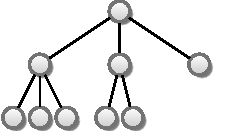
\includegraphics{images/tree_complete.pdf}}\hfill%
  \subfigure[min depth]{\label{subfig:treeMinDepth}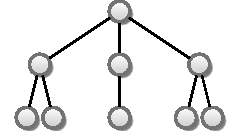
\includegraphics{images/tree_mindepth.pdf}}\hfill%
  \subfigure[full tree]{\label{subfig:treeFull}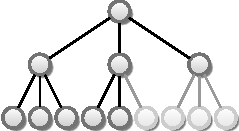
\includegraphics{images/tree_full.pdf}}%
}{Box with gray background intended to hold subfigures}{fig:trees}


%%
\section{Tables}\label{sec:tables}

Unfortunately, tables can be a pain in \LaTeX{} and have a clear tendency to look ugly. For this reason, we built the package \emph{tuhhtable}. A brief discussion of frequently used table pattern follow in dedicated subsections. 


\subsection{Simple Tables with Headings}\label{sub:simpleTables}

When creating tables, a couple of rules should be obeyed. Firstly, vertical lines are rarely helpful in tables. In contrast, they make a table harder to read in most cases, when people read from left to right. So try not to use them. To further support readability---while also hinting at eye candy---shaded rows are employed. To mark the end of a table and to separate the table body from the header, horizontal lines can be used. A recommended table layout is depicted in Table~\ref{tbl:simple}. Have a look at the source code of this document to understand how things work.

\begin{tuhhtable}
  \begin{tabular}[tp]{L{.3\textwidth}C{.3\textwidth}R{.3\textwidth}}
    \THc{1}{c}{Head 1} & \THc{1}{c}{Head 2} & \THc{1}{c}{Head 3} \\
    \THsub{1}{c}{sub 1} & \THsub{1}{c}{sub 2} & \THsub{1}{c}{sub 3} \\
    \abovebodyrule
    l1     & c1     & r1     \\\TRc
    l2     & c2     & r2     \\
    l3     & c3     & r3     \\\TRc
    \belowbodyrule
  \end{tabular}
  \caption{A simple table with a heading}
  \label{tbl:simple}
\end{tuhhtable}


\subsection{Special Table Elements}\label{sub:specialTableElements}

In case your are carrying out comparisons of, lets say, different algorithms, you might want to judge the quality of certain properties by symbols, such as '+', '-', or the like. Unfortunately, these symbols are not very fancy, so that we have defined a set of more eye-catchings ones. They are displayed in Table~\ref{tbl:elements}. Again, have a look at the source code of this document to understand how they can be used.

\begin{tuhhtable}
  \footnotesize\centering
  \begin{tabular}[tp]{L{.22\textwidth}C{.22\textwidth}C{.22\textwidth}C{.22\textwidth}}
    \THempty & \THc{1}{c}{Product 1} & \THc{1}{c}{Product 2} & \THc{1}{c}{Product 3} \\
    \abovebodyrule
    \TRh{1}{l}{has feature}  & \tblYes    & \tblYes  & \tblNo    \\\TRc
    \TRhc{1}{l}{usability}   & \tblGood   & \tblBest & \tblBad   \\
    \TRh{1}{l}{price}        & \tblNA     & \tblFair & \tblWorst \\\TRc
    \belowbodyrule
  \end{tabular}
  \caption{Special symbols for use in tables}
  \label{tbl:elements}
\end{tuhhtable}



\subsection{Advanced Tables}\label{sub:advancedTables}

Sometimes, a simple table layout as presented in the previous section is not sufficient. An example is shown in Table~\ref{tbl:advanced}. Hence, additional commands are available. 

% DECISION GUIDANCE TABLE
\begin{sidewaystable}
  \footnotesize\centering
  \begin{tabular}[htp]{lC{3.2cm}C{3.2cm}C{3.2cm}C{3.3cm}C{3.2cm}}
  \THempty    & \THc{1}{c}{Type I}   &
                 \THc{1}{c}{Type II}  &
                  \THc{1}{c}{Type III} &
                   \THc{1}{c}{Type IV}  &
                    \THc{1}{c}{Type V}  \\
%
  \TRx{6}{l}{Network Size}\\
  \abovebodyrule
  Small       & \tblWorst    & \tblGood     & \tblBest     & \tblBest     & \tblBad      \\\TRc
  Medium      & \tblFair     & \tblFair     & \tblGood     & \tblFair     & \tblFair     \\
  Large       & \tblBad      & \tblWorst    & \tblWorst    & \tblWorst    & \tblBest     \\
  \belowbodyrule
%
  \TRx{6}{l}{Density}\\
  \abovebodyrule
  Low         & \tblWorst    & \tblFair     & \tblBad      & \tblWorst    & \tblBad      \\\TRc
  Medium      & \tblFair     & \tblFair     & \tblFair     & \tblFair     & \tblGood     \\
  High        & \tblWorst    & \tblFair     & \tblGood     & \tblFair     & \tblGood     \\
  \belowbodyrule
%
  \TRx{6}{l}{Initial Fill Level}\\
  \abovebodyrule
  Low         & \tblFair     & \tblGood     & \tblBest     & \tblBest     & \tblGood     \\\TRc
  High        & \tblBad      & \tblBad      & \tblWorst    & \tblWorst    & \tblBest     \\
  \belowbodyrule
%
  \TRx{6}{l}{Variation of Initial Fill Levels}\\
  \abovebodyrule
  Low         & \tblBest     & \tblGood     & \tblBad      & \tblGood     & \tblBest     \\\TRc
  High        & \tblBest     & \tblBad      & \tblWorst    & \tblGood     & \tblBest     \\
  \belowbodyrule
%
  \TRx{6}{l}{Collisions and Packet Loss}\\
  \abovebodyrule
  Collisions / Yield &
    \tblYes / \tblWorst &
    \tblNo  / \tblBest &
    \tblNo  / \tblBest &
    \tblNo  / \tblBest &
    \tblYes / \tblFair     \\\TRc
  Packet Loss & \tblGood     & \tblFair     & \tblWorst    & \tblWorst    & \tblGood     \\
  \belowbodyrule
  \end{tabular}
  \caption{Characteristics of the TDMA schedules: Decision Guidance \cite{Renner:2008:Diploma}}
  \label{tbl:advanced}
\end{sidewaystable}



\section{Enumerations \& Co.}\label{sec:enumerations}

Feel free to use enumerations, itemizations, and the like to suit your needs. We have adjusted the itemization to match our slides class plus our color scheme. We thus discourage you from changing items or colors.



\section{Listings}\label{sec:listings}

For placing and typesetting listings, we encourage the use of the \emph{listings} package available for \LaTeX. Please have a look into the corresponding package manual. The facilitate the usage of this package, we have already set it up to follow the same look as the rest of our visual stuff. This includes the gray background, the frame, and appropriate colors. The package is automatically loaded by the template class and defines \emph{C++} as the default programming language---you are completely free to adjust the language, of course. A sample listing is displayed in Lst.~\ref{lst:sampleListing}. Note that all listings should have labels with the prefix \cmd{lst:} and should be referenced in the text. Besides complete listings, we have defined the command \cmd{\textbackslash{}cmd}, which display its first parameter text in monospace font.

\begin{tuhhlisting}[label=lst:sampleListing,caption={A simple C++ program for reading in positions},language=C++]
#include <iostream>                                                                       
#include <vector>                                                                         
#include <inttypes.h>                                                                     

using namespace std;

/* 2-D positions */
typedef struct pos_s {
        int16_t  x, y;
} pos_t;

int main(void)
{
        uint16_t       numData;
        vector<pos_t>  v;
        pos_t          tmp;

        /* read numData 2-D points */
        cin >> numData;
        for (unsigned i = 0; i < numData; i++) {
                cin >> tmp.x >> tmp.y;
                v.push_back(tmp);
        }
        cout << "read " << numData << " points" << endl;

        /* process data */
        process(v);

        return 0;
}
\end{tuhhlisting}

%\chapter{Style Guide}\label{cha:styleGuide}

Finally, we want to give some advices and recommendations on styling. This does not relate to writing skills, which is gracefully embraced by the \emph{Chicago Writer's Manual}.


\section{Fonts}\label{sec:fonts}

Font setup etc. has been done for you by means of this very template. We hence expect you to follow the given style; meaning that we discourage you from changing font sizes, faces, families, colors, as well as line and paragraph spacing or any spacing in general.


\section{Citing and Referencing}\label{sec:citeAndRef}

Citing other sources and referencing parts of your work is quite easy using the commands \cmd{\textbackslash{}cite} and \cmd{\textbackslash{}ref}. Yet, let us mention some aspects. Firstly, when citing, you should make clear, somehow, which part is from the cited work and which is not. Secondly, you most likely want to place a tilde ($\sim$) between the word just in front of the \cmd{\textbackslash{}cite} or \cmd{\textbackslash{}ref} commands to avoid ugly looking line breaks. Thirdly, note that citations and references are proper parts of a sentence: Do not simply put them at the end of a sentence; use them as nouns!

More importantly, obey the following rules. Always capitalize when referencing, e.g., say Fig.~17 instead of fig.~17. You can abbreviate Figure with Fig., Section with Sect., and Listing with Lst. When referencing equations, simply place the number in parentheses---e.g., say (3.2) instead of Eq.~3.2---that's all. While you can certainly do this by hand, we encourage you to use the \emph{cleveref} package, which already does this for you. By using \cmd{\textbackslash{}cref} or \cmd{\textbackslash{}Cref} (at the beginning of a sentence) as a replacement for \cmd{\textbackslash{}ref}, the type of reference is automatically added. Please check the manual of the package for further details.

For your own sake, use a pattern for labels. We recommend to use prefixes for each type of label: chapters (\cmd{cha:}), sections (\cmd{sec:}), subsections and below (\cmd{sub:}), figures (\cmd{fig:}), tables (\cmd{tbl:}), listings (\cmd{lst:}), and equations (\cmd{eqn:}).


\section{Physical Units}\label{sec:siunits}

If you plan on using physical units, particularly SI-units, in your report, we encourage you to use the \emph{siunitx} package for \LaTeX. In all cases, separate numbers from their units with a small space, i.e., with a \cmd{\textbackslash{},}. Well, there is an exception: No space for~\%!


\section{Mathematical Stuff}

When using mathematical functions or sub-/superscripts that are text and not variables, please typeset these appropriately: In the case of functions, use the command version, e.g., \cmd{\textbackslash{}log} (prints $\log$) instead of plainly \cmd{log} (which prints $log$). For subscripts or the like, use the command \cmd{\textbackslash{}textnormal}. Compare $T_{sleep}$ with $T_\textnormal{sleep}$. The reasons for this is twofold. Firstly, the produced italic text looks ugly, and secondly, italics are used for variables (only).

The usage of the environment \cmd{equation} is disouraged and may cause display errors. In the future, please use the \cmd{align} environment for equations:

\begin{align*}
	|x|= 
	\begin{cases} 
			x 	& \text{if $x > 0 $,} \\
			-x 	& \text{if $x \leq 0$.}
	\end{cases}
\end{align*}

\begin{tuhhlisting}[language=TeX]
\begin{align*}
	|x|= 
	\begin{cases} 
			x 	& \text{if $x > 0 $,} \\
			-x 	& \text{if $x \leq 0$.}
	\end{cases}
\end{align*}
\end{tuhhlisting}



\section{Bibliography}\label{sec:bib}

When it comes to writing your bibfile, i.e., your bibliography, please follow the next few advices. Firstly, be consistent (if possible): Regarding authors' names, either abbreviate first names always or write them out always! For US addresses, write down the name of the city, the two-character abbreviation for the state plus the term USA! For all other countries, the name of the city and the country are sufficient. Capitalize titles correctly (there are multiple rules on this, please pick one and stick to it)! If possible, write down the full name of a conference and repeat its abbreviation with the year in parentheses afterwards. We give a few examples in the following listings.

Beside this, please have a look at the required fields for the main types of citations:
\begin{description}
  \item[Journal Articles] Use the type \cmd{@article} and include the fields \cmd{author}, \cmd{title}, \cmd{journal}, \cmd{volume}, \cmd{number}, \cmd{year}, \cmd{publisher}, and \cmd{address}.
  \item[Conference Papers] Use the type \cmd{@inproceedings} and provide the fields \cmd{author}, \cmd{title}, \cmd{booktitle}, \cmd{month}, \cmd{year}, and \cmd{address}.
  \item[Technical Reports] Use the type \cmd{@techreport} and provide the fields \cmd{author}, \cmd{title}, \cmd{month}, \cmd{year}, and \cmd{institution}.
  \item[Websites] Use the type \cmd{@misc} and provide the fields \cmd{author}, \cmd{title}, \cmd{year}, \cmd{note} and \cmd{howpublished}. The last two fields hold a note on your last visiting date of the site and its web address.
\end{description}

We have put together a couple of examples for you in Lst.~\ref{lst:sampleBibtex}.

\begin{tuhhlisting}[label=lst:sampleBibtex,language=TeX,caption={BibTeX examples},{morekeywords={@article,@inproceedings,@techreport,@misc}},{morestring=[b]"}]
@article{ ECPS:2002:ConnectingThePhysicalWorld,
	author       = "D. Estrin and D. Culler and K. Pister and G. Sukhatme",
	title        = "{Connecting the Physical World with Pervasive Networks}",
	journal      = "IEEE Pervasive Computing",
	volume       = "1",
	number       = "1",
	year         = "2002",
	publisher    = "IEEE Educational Activities Department",
	address      = "Piscataway, NJ, USA"
}

@inproceedings{ KPC:2006:StructuralMonitoring,
	author       = "S. Kim and S. Pakzad and D. Culler and J. Demmel and G. Fenves and S. Glaser and M. Turon",
	title        = "{Wireless Sensor Networks for Structural Health Monitoring}",
	booktitle    = "Proceedings of the 4th International Conference on Embedded Networked Sensor Systems (SenSys~'06)",
	month        = oct,
	year         = "2006",
	address      = "Boulder, CO, USA"
}

@techreport{ EV:2005:TDMAScheduling,
	author       = "S. Coleri Ergen and P. Varaiya",
	title        = "{TDMA Scheduling Algorithms for Sensor Networks}",
	year         = "2005",
	month        = jul,
	institution  = "Department of Electrical Engineering and Computer Science, University of California, Berkeley, CA, USA"
}

@misc{ TI5:WIKI,
	author       = "S. Untersch{\"u}tz",
	title        = "{Network Simulator (NS-2), Institute of Telematics, Hamburg University of Technology, Germany}",
	howpublished = "http://wiki.ti5.tu-harburg.de/wsn/ns2/intro",
	year         = 2008,
	note         = "Last visited: 05/06/2008"
}
\end{tuhhlisting}



% Bibliography
% if you have cited papers that are not referenced, but important for your work,
% uncommented the following line; however, this should generally by unnecessary
% and hints at improper citing.
%\nocite{*}
\tuhhbibliography{thesis}


% Appendix
% Feel free to add additional appendix chapters (e.g., measurement setups, etc.)
\begin{tuhhappendix}
  \chapter{Content of the DVD}

In this chapter, you should explain the content of your DVD. 

\end{tuhhappendix}


% The End
\end{document}
